\block{\begin{blockbody}\section{Why do we need bioimage analysis?}
	\tfont
    We tend to judge data volumes based on their size on a hard drive, but it is worth considering what a typical image actually represents - a numerical matrix with millions of entries, all of which cannot possibly be interrogated manually:\par
     \begin{minipage}{0.72\textwidth}
	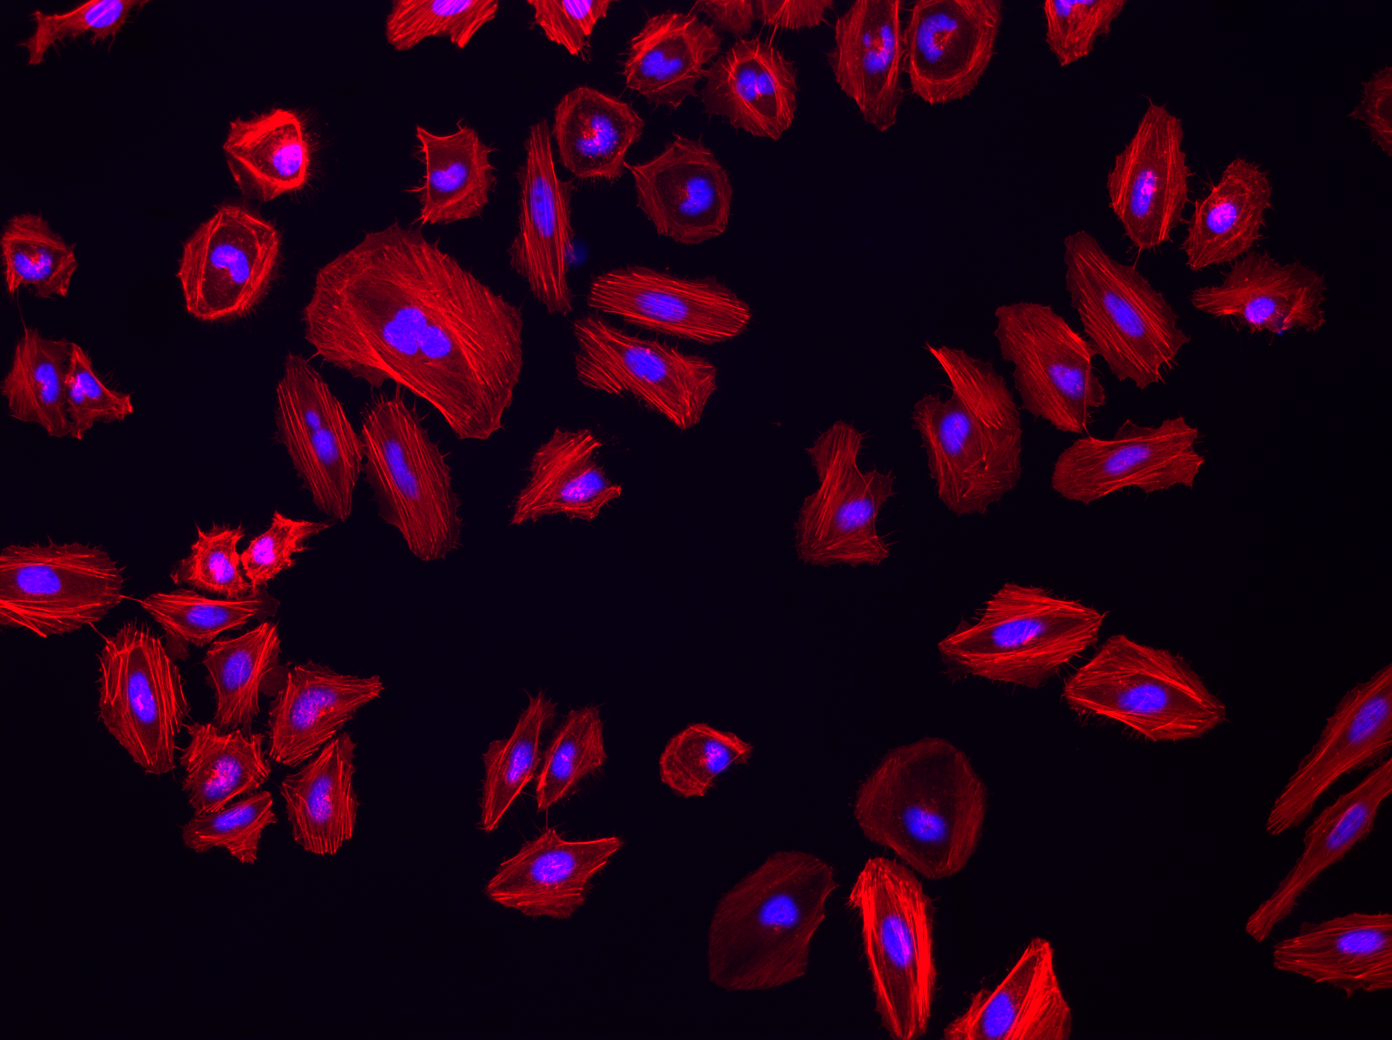
\includegraphics[height=0.07\textheight]{DAPIActin} \hfill 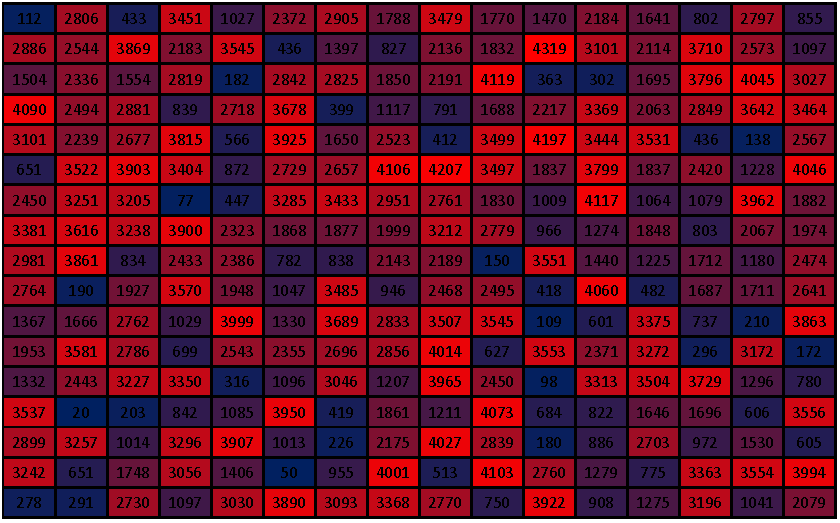
\includegraphics[height=0.07\textheight]{ImageMatrix} \par
    \end{minipage}\hfill
    \begin{minipage}[c][0.25\textwidth][c]{0.23\textwidth}
    	\setlength{\unitlength}{0.9\textwidth}
    	\begin{picture}(1.0, 1.2)%
	\put(0.1,0.3){\fcolorbox{black}{white}{\parbox[b][0.7\unitlength][c]{0.7\unitlength}{\centering\textbf{4 Million Data Points}}}}%
	\put(0.05,0.35){\rotatebox{90}{\makebox(0,0)[lb]{\smash{2048 Pixels}}}}
	\put(0.33,0.03){\makebox(0,0)[lb]{\smash{2048 Pixels}}}
\end{picture}\par
    \end{minipage} \par
    	Experiments can entail hundreds of such exposures of potentially millions of cells. Manual analysis is laborious and time-consuming and effectively places an upper limit on the volume of data that can be \lq\lq processed''. This, in turn, places severe limitations on the scale of experiments that can be conducted, thus limiting scientific advancement.\par
    	{\centering\begin{tikzpicture}[every node/.style={inner sep=0}]
 	\node (system) at (1.0, 0.0) {
\includegraphics[height=0.18\textwidth]{Microscope}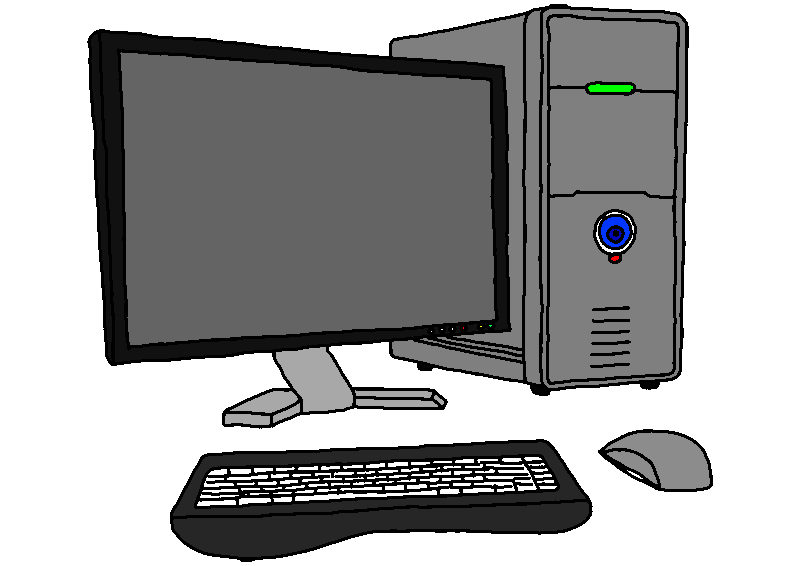
\includegraphics[height=0.18\textwidth]{Computer}};
    \node (server) at (4.0 * \dist, 0.0) {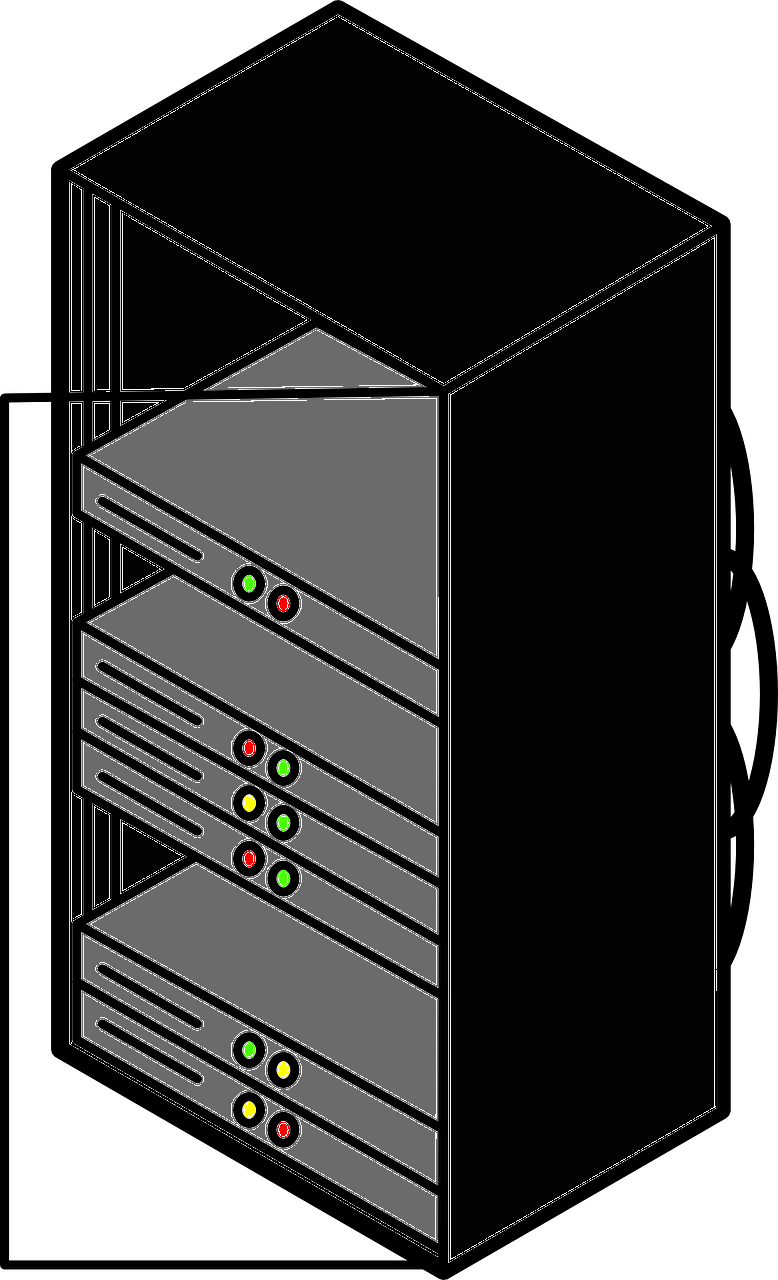
\includegraphics[height=0.22\textwidth]{Server}};
    \node (elbowa) at (5.25*\dist, 0.0) {};
    \node (elbowb) at (5.25*\dist, -0.65 * \dist) {};
    \node (elbowc) at (5.25*\dist, 0.85 * \dist) {};
    \node (cassette) at (7.35 * \dist, -0.65 * \dist) {
\includegraphics[height=0.165\textwidth]{Cassette}};
    \node[block] (steady) at (7.35 * \dist, 0.85 * \dist) {\textbf{Steady State: 365TB}};
	\path[arrow] (system) -- (server);
	\path[arrow] (server) -- (elbowa) -- (elbowb) -- (cassette);
    \path[arrow] (server) -- (elbowa) -- (elbowc) -- (steady);
    \node (label1) at (2.8 * \dist, 0.15 * \dist) {\lfont 1 TB / Day};
    \node (label2) at (5.35 * \dist, -0.8 * \dist) {\lfont After 12 Months};
\end{tikzpicture}\par}\par
    	There is also a strong economic argument for bioimage analysis. A typical 1PB server costs approximately \textsterling 100K and consumes \textasciitilde 10kW, which equates to \textasciitilde\textsterling 10K per annum. Reliance on manual analysis is therefore not cost-effective, as most of the data stored will never be analysed. Automated analysis is essential to unleash the full scientific potential of modern microscopy. There is a growing acceptance of this need in the community. For example, in their recent strategic review of bioimaging \citep{bbsrc2018}, the BBSRC concluded that:\par
        \centering\fcolorbox{dblue}{lblue}{\parbox{0.85\textwidth}{\color{dblue}\lq\lq Data skills and training are required across the biosciences community to enable high-quality quantitative bioimaging. This includes theoretical understanding of image analysis as well as practical skills and expertise.''}}\par
\end{blockbody}}